\documentclass[UTF8]{ctexrep}

\usepackage{fancyhdr}
\usepackage[letterpaper, left=1in, right=1in, top=1in, bottom=1in]{geometry}
\usepackage{sectsty}
\usepackage{graphicx}
\usepackage{subfig}
\usepackage[section]{placeins}
\usepackage{hyperref}
\usepackage{amsmath}
\usepackage{listings}
\usepackage{color}

\definecolor{dkgreen}{rgb}{0,0.6,0}
\definecolor{gray}{rgb}{0.5,0.5,0.5}
\definecolor{mauve}{rgb}{0.58,0,0.82}

\lstset{frame=tb,
  language=C,
  aboveskip=3mm,
  belowskip=8mm,
  showstringspaces=false,
  columns=flexible,
  basicstyle={\small\ttfamily},
  numbers=none,
  numberstyle=\tiny\color{gray},
  keywordstyle=\color{blue},
  commentstyle=\color{dkgreen},
  stringstyle=\color{mauve},
  breaklines=true,
  breakatwhitespace=true,
  tabsize=3
}

\hypersetup{
    colorlinks=true,
    linkcolor=blue,
    filecolor=magenta,
    urlcolor=cyan,
}
\allsectionsfont{\mdseries\scshape}

\renewcommand{\thesection}{\arabic{section}}

\newcommand{\horrule}[1]{\rule{\linewidth}{#1}}
\title{
    \horrule{0.5pt} \\[0.4cm]
    \huge Project 1 \\
    \horrule{2pt}
}
\author{
    陈思贝 (718030290013)
}
\date{
    % TODO: Date
}

\begin{document}
    \maketitle
    \section{实验过程}
    所有模块均写在同一个c文件\lstinline{homework1.c}中。\\
    
    \subsection{Module 1}
    模块1实现过程较为简单,仅需在\lstinline{__init}和\lstinline{__exit}中适当的位置加入以下指令即可。
    \begin{lstlisting}
        printk(KERN_INFO "Hello, world\n");
        printk(KERN_INFO "Goodbye, world\n");
    \end{lstlisting}

    \subsection{Module 2}
    对模块2的实现需要预先定义以下变量。
    \begin{lstlisting}
        static int paramInt;
        static char *paramStr;
        static int paramArr[3];
        static int pr_arr;
    \end{lstlisting}

    然后通过\lstinline{module_param}从传入参数中接收变量。其中\lstinline{int}和\lstinline{charp}(字符串)可直接
    传入,数组则可用专门的\lstinline{module_param_array}进行接收,需要提前确定数组的个数并指定大小。
    \begin{lstlisting}
        module_param(paramInt, int, 0644);
        module_param(paramStr, charp, 0);
        module_param_array(paramArr, int, &pr_arr, 0444);
    \end{lstlisting}

    输出传入参数的过程与模块1的进程类似。
    \begin{lstlisting}
        printk(KERN_INFO "Param-int:%d;\n", paramInt);
        printk(KERN_INFO "Param-str:%s;\n", paramStr);
        for (i = 0; i < (sizeof paramArr / sizeof (int)); i++) {
            printk(KERN_INFO "Param-arr[%d]: %d\n", i, paramArr[i]);
        }
    \end{lstlisting}

    \subsection{Module 3}
    模块3的实现难度大了许多,在\lstinline{\proc}中创建文件以及退出时移除文件只需以下指令:
    \begin{lstlisting}
        proc_create("test", 0, NULL, &hello_proc_fops);
        remove_proc_entry("test", NULL);
    \end{lstlisting}
    
    重点在于\lstinline{hello_proc_fops}的类型从\lstinline{file_operations}变成了\lstinline{proc_ops}。
    因此要对课件中的实现过程稍作更改:
    \begin{lstlisting}
        static const struct proc_ops hello_proc_fops = {
            .proc_open = hello_proc_open,
            .proc_release = single_release,
            .proc_read = seq_read,
            .proc_lseek = seq_lseek
        };
    \end{lstlisting}

    因为建立的是只读文件,需要对打开文件时的操作进行定义,实现方法如下:
    \begin{lstlisting}
        static int hello_proc_show(struct seq_file *m, void *v) {
            seq_printf(m, "Hello proc!\n");
            return 0;
        }

        static int hello_proc_open(struct inode *inode, struct  file *file) {
            return single_open(file, hello_proc_show, NULL);
        }
    \end{lstlisting}

    \subsection{Module 4}
    模块4的难点在于对读写文件的读写功能的实现。创建和移除文件夹以及读写文件实现方法如下:
    \begin{lstlisting}
        static struct proc_dir_entry *dir;

        dir = proc_mkdir("hello_dir", NULL);
        proc_create("test", 0660, dir, &hello_fops);

        remove_proc_entry("test", dir);
        remove_proc_entry("hello_dir", NULL);
    \end{lstlisting}

    与模块3一样,模块4中也用到了最新的\lstinline{proc_ops}类型。读的实现与模块3基本一致。写的功能通过\lstinline{copy_from_user}实现。
    从用户的内存中把字符串复制进入内核的内存中,并在读取该字符串的时候将其提供给读取模块。
    \begin{lstlisting}
        static char *str = NULL;

        static ssize_t hello_write(struct file *file, const char __user *buffer, size_t count, loff_t *f_pos) {
            char *tmp = kzalloc((count+1),GFP_KERNEL);
            if(!tmp) return -ENOMEM;
            if(copy_from_user(tmp,buffer,count)){
                kfree(tmp);
                return -EFAULT;
            }
            kfree(str);
            str=tmp;
            return count;
        }

        static int hello_show(struct seq_file *m, void *v) {
            seq_printf(m, "%s\n", str);
            return 0;
        }

        static int hello_open(struct inode *inode, struct file *file) {
            return single_open(file, hello_show, NULL);
        }

        static const struct proc_ops hello_fops = {
            .proc_open = hello_open,
            .proc_release = single_release,
            .proc_read = seq_read,
            .proc_write = hello_write,
            .proc_lseek = seq_lseek
        };
    \end{lstlisting}

    \section{实验效果截图}
    \begin{figure}[h!]
        \centering
        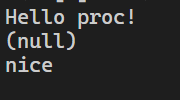
\includegraphics{output_screenshot.png}
        \caption{输出内容截图}
    \end{figure}
    \begin{figure}[h!]
        \centering
        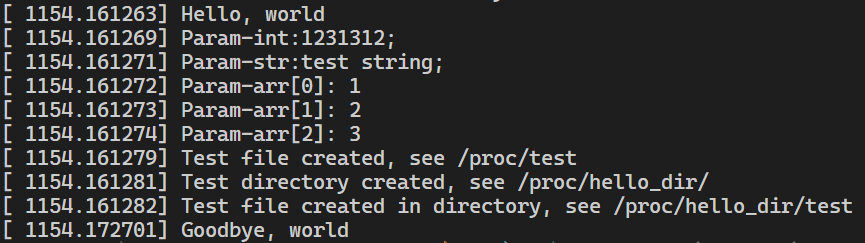
\includegraphics{log_screenshot.png}
        \caption{内核日志截图}
    \end{figure}

    \section{实验心得}
    本次实验掌握了针对内核进程最基础的操作:写入内核日志,读取传入的参数,在\lstinline{\proc}中创建不同权限的文件和文件夹,
    以及对于可读写文件的实现。同时也对模块的加载和卸载环节以及\lstinline{Makefile}有着更为深刻的了解。为接下来的内核模块
    编程打下了基础。
\end{document}